\section{Resultaten}
In deze sectie tonen en bespreken we de bekomen resultaten.

\subsection{Rauwe Data}
\subsubsection{Weinig Snijpunten}
\begin{figure}[H]
   \centering
   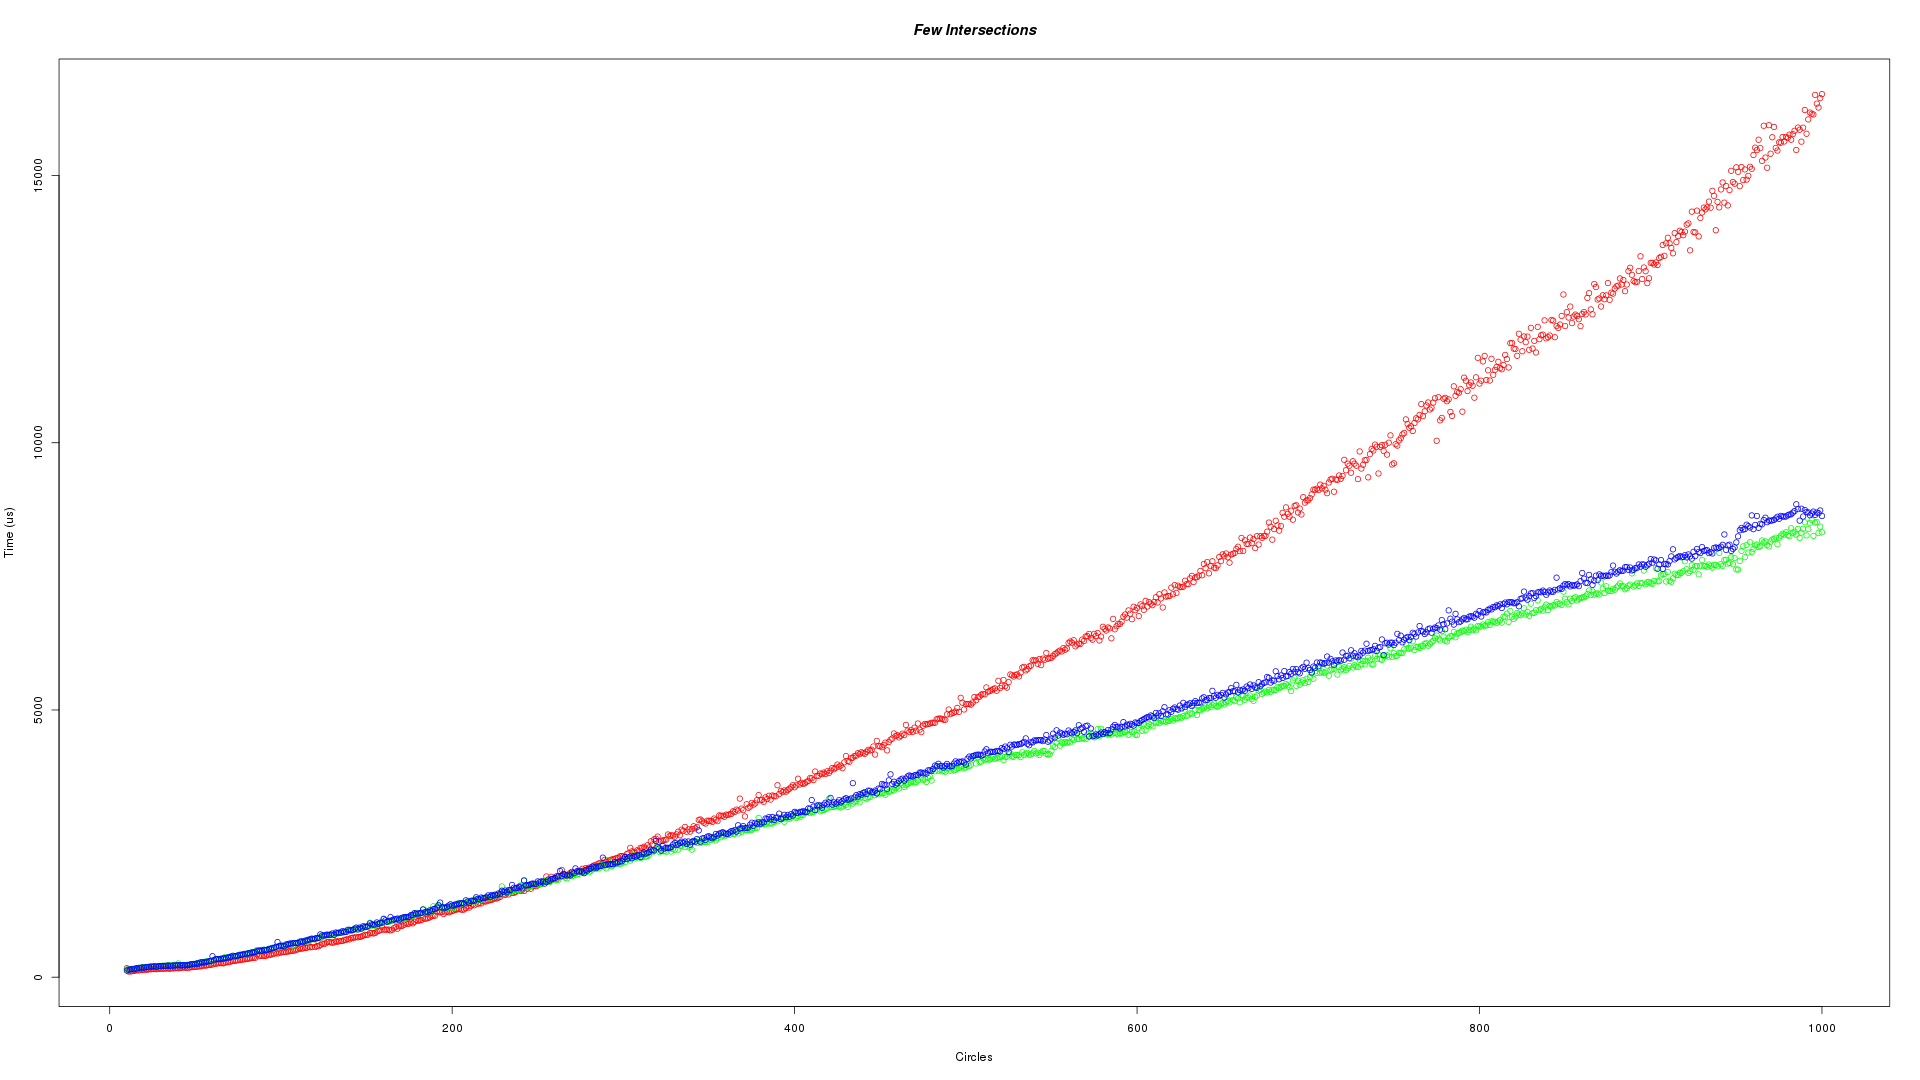
\includegraphics[width=\textwidth]{illustraties/fewIntersections.png}
\end{figure}
   
\subsubsection{Veel Snijpunten}
\begin{figure}[H]
   \centering
   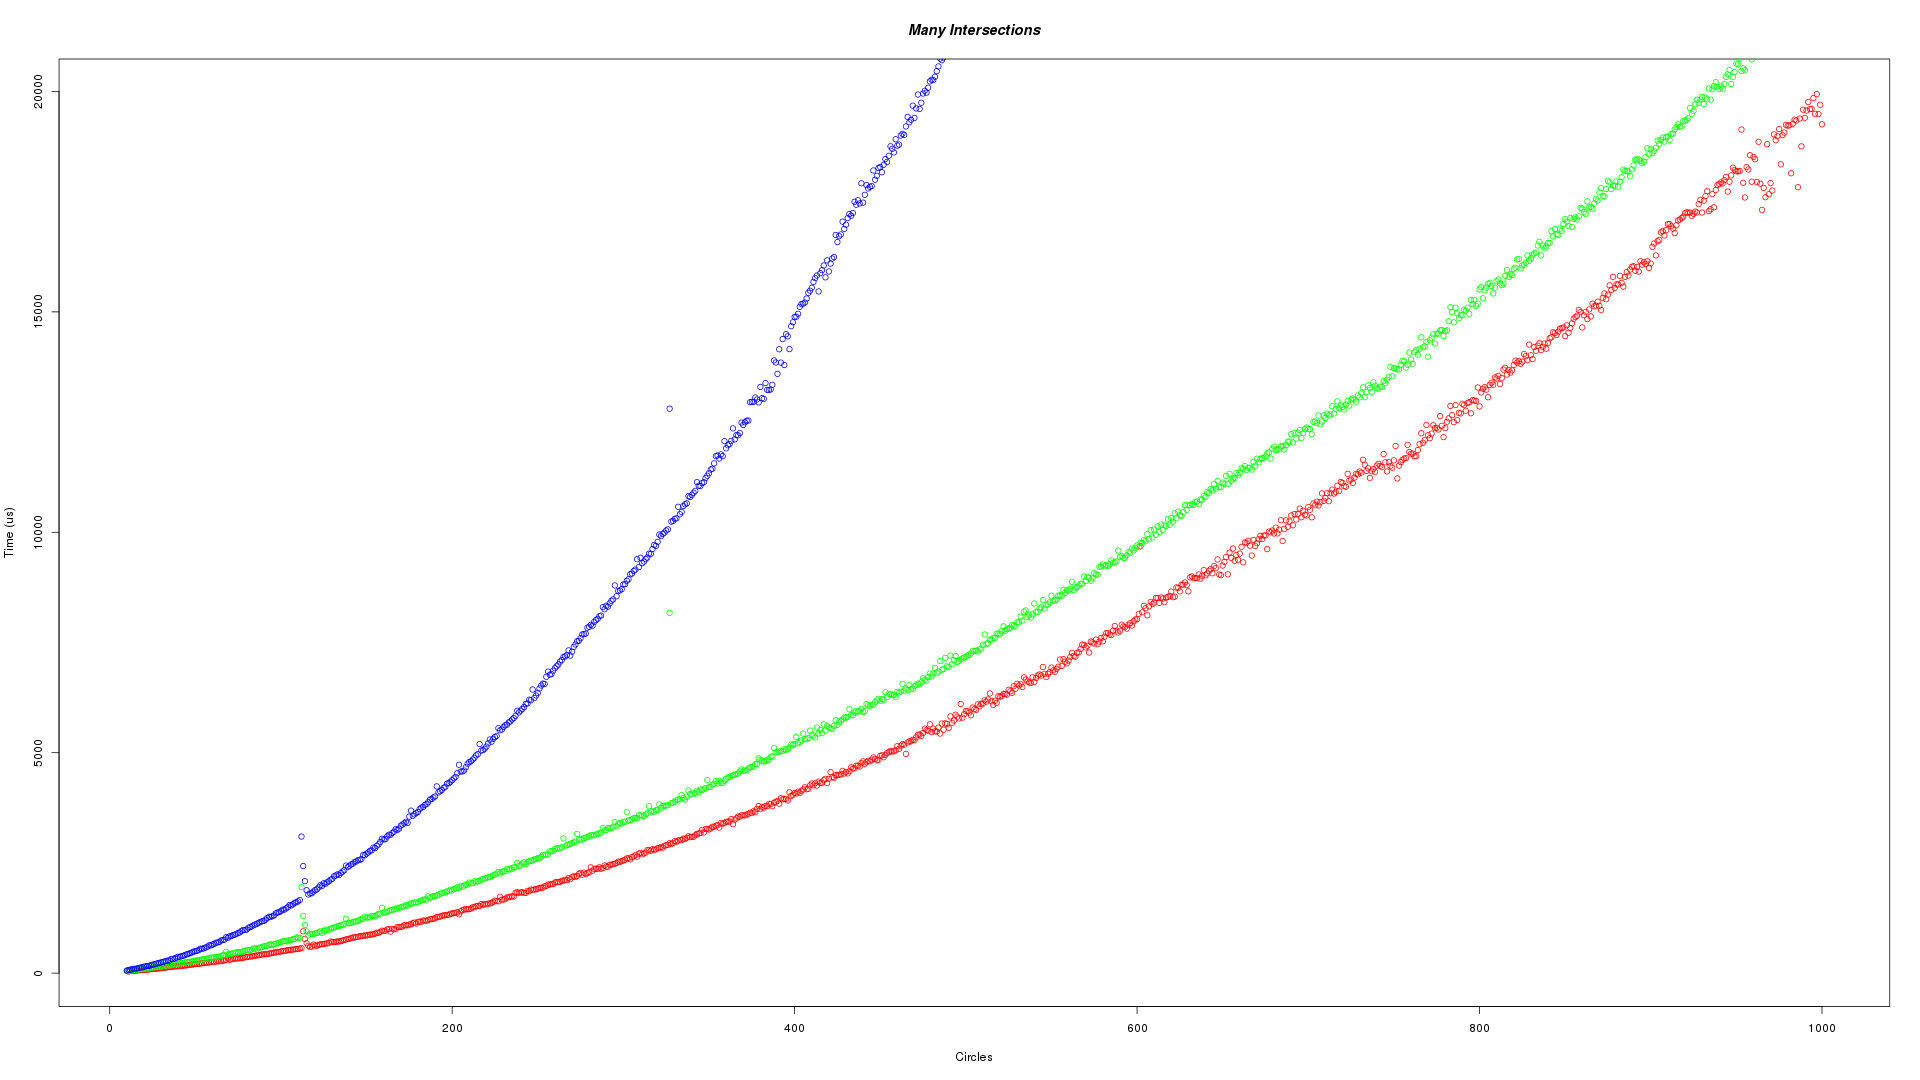
\includegraphics[width=\textwidth]{illustraties/manyIntersections.png}
\end{figure}

\subsubsection{3D plot}
\begin{figure}[H]
   \centering
   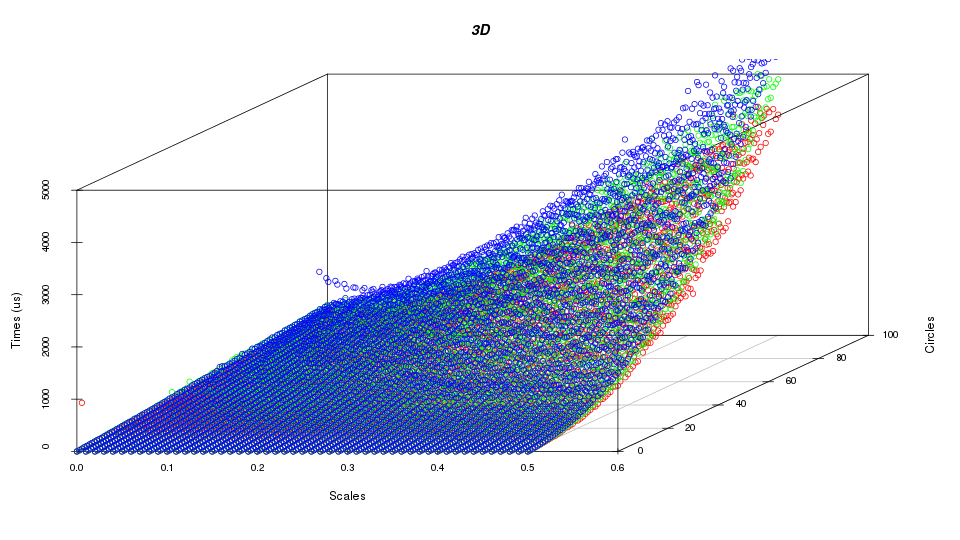
\includegraphics[width=\textwidth]{illustraties/3DScatter.png}
\end{figure}

\subsection{Doubling Ratio}
\subsubsection{Naief}
\begin{figure}[H]
\[
\begin{array}{|c||ccccccc|}
\hline 
& 20 & 40 & 80 & 160 & 320 & 640 & 1280\\
\hline \hline 
0.000 & 3.4 & 3.9 & 4.6 & 4.2 & 4.3 & 4.3 & 4.2 \\ \hline 
0.001 & 3.2 & 4.3 & 4.2 & 4.9 & 4.1 & 4.3 & 4.2 \\ \hline 
0.500 & 3.5 & 4.0 & 4.5 & 4.8 & 4.9 & 4.8 & 5.0 \\ \hline 
1.000 & 3.4 & 4.2 & 4.5 & 4.7 & 5.3 & 5.3 & 5.3 \\ \hline 
\end{array}
\]


\label{doublingratio_1}
\caption{Doubling ratio 1}
\end{figure}

\subsubsection{Kwadratisch}
\begin{figure}[H]
\[
\begin{array}{|c||ccccccc|}
\hline 
& 20 & 40 & 80 & 160 & 320 & 640 & 1280\\
\hline \hline 
0.000 & 1.8 & 2.3 & 2.2 & 2.3 & 2.1 & 2.2 & 2.1 \\ \hline 
0.001 & 2.0 & 2.4 & 2.1 & 2.5 & 2.2 & 2.3 & 2.6 \\ \hline 
0.500 & 3.1 & 3.9 & 4.2 & 4.3 & 5.1 & 5.2 & 5.1 \\ \hline 
1.000 & 3.7 & 4.3 & 4.0 & 4.7 & 5.5 & 5.1 & 5.4 \\ \hline 
\end{array}
\]


\label{doublingratio_2}
\caption{Doubling ratio 2}
\end{figure}

\subsubsection{Linearitmisch}
\begin{figure}[h]
\[
\begin{array}{|c||ccccccc|}
\hline 
& 20 & 40 & 80 & 160 & 320 & 640 & 1280\\
\hline \hline 
0.000 & 2.2 & 2.2 & 2.2 & 2.3 & 2.2 & 2.1 & 2.2 \\ \hline 
0.001 & 2.1 & 2.2 & 2.2 & 2.3 & 2.8 & 1.8 & 2.4 \\ \hline 
0.500 & 3.3 & 3.4 & 4.1 & 4.4 & 5.2 & 5.2 & 5.0 \\ \hline 
1.000 & 3.4 & 4.0 & 4.2 & 4.6 & 5.5 & 5.1 & 5.1 \\ \hline 
\end{array}
\]


\label{doublingratio_3}
\caption{Doubling ratio 3}
\end{figure}
